
% ********** Chapter 9 **********
\chapter{Java ME Client}
\label{sec:JavaMEClient}

The Java ME Client is a client of web service interface which described in chapter \nolinebreak \ref{sec:WebServiceInterface}. It implemented all of the interfaces of web service of Web Call SDK. Besides the web service interface, Java ME Client also provide some convenient function such as load contact book from mobile phone and synchronize it with Web Call SDK server. 

\section{Architecture}
\label{sec:JavaMEClient:Architecture}

The architecture of Java ME web service client is shown in Figure \nolinebreak \ref{fig:TheArchitectureOfJavaMEClient}. It can be seen from the diagram that there are three layers in the Java ME client. They are, from bottom to top, Java ME API, Business Logic and User Interface. 

\begin{figure}[!hbtp]
\centering
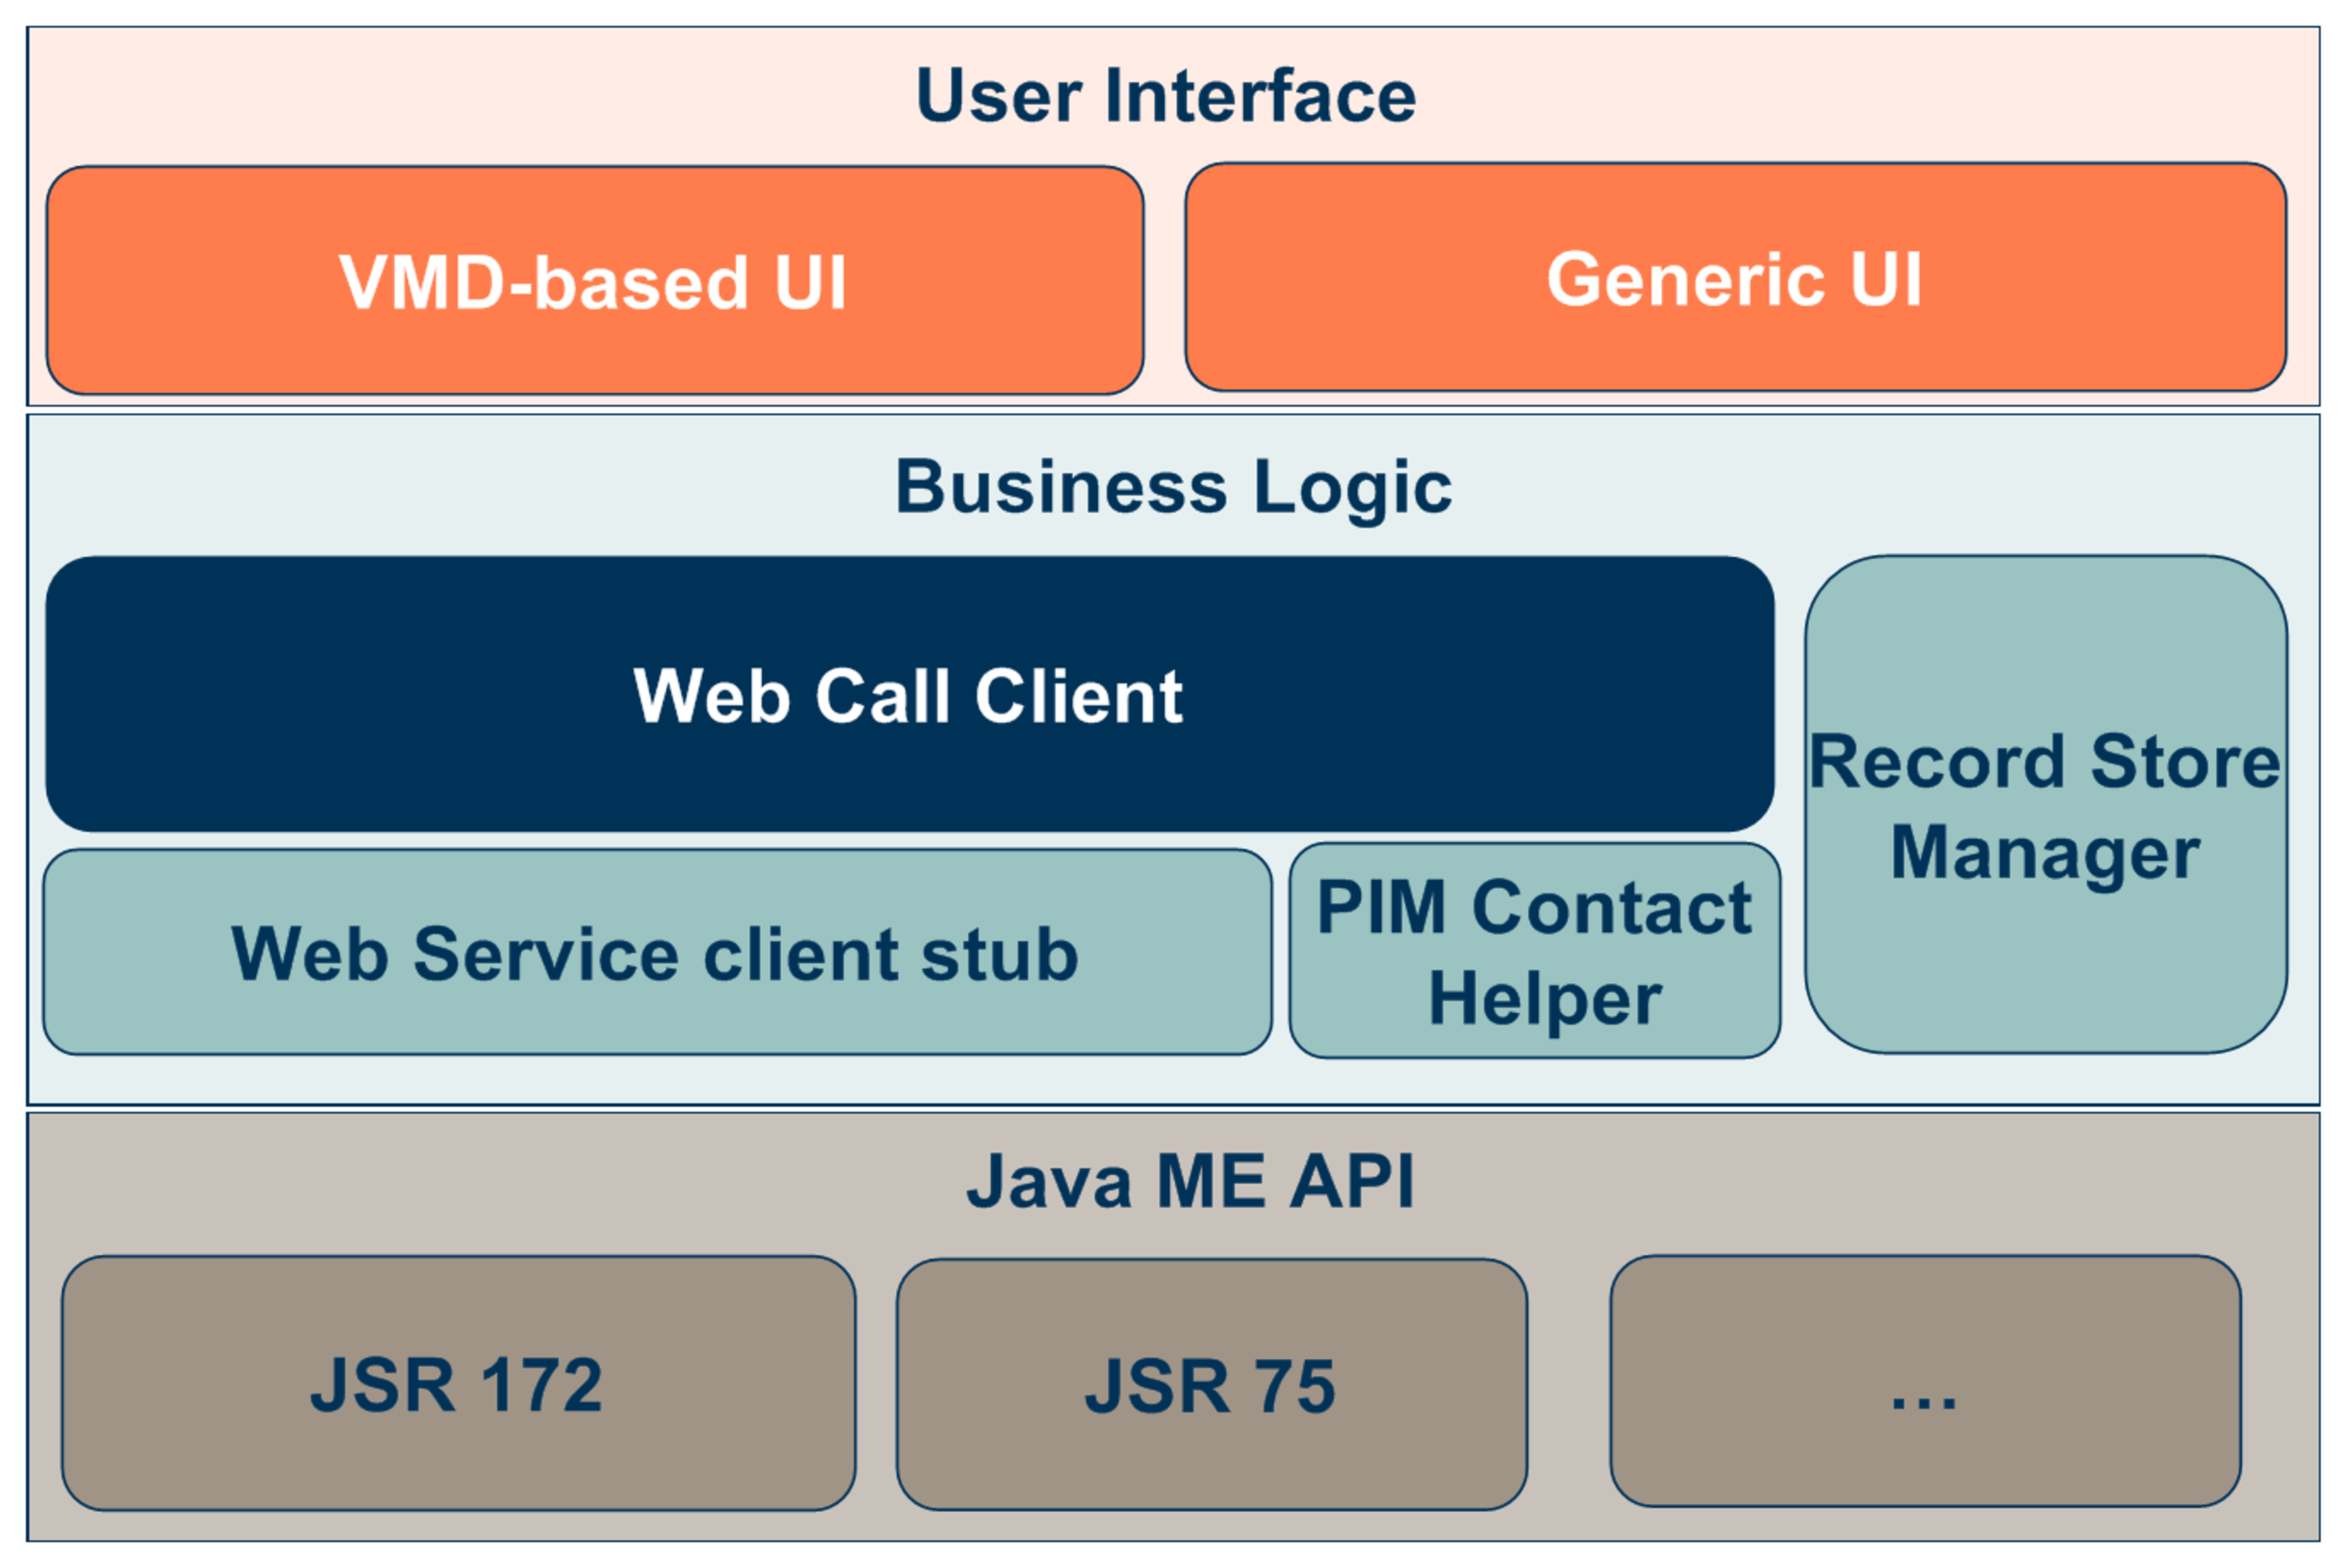
\epsfig{file=chap09/resources/java_me_client_architecture, width=5.2in}
\caption{The Architecture of Java ME Client}
\label{fig:TheArchitectureOfJavaMEClient}
\end{figure}

The Java ME API layer is the standard API set for Java ME platform. To meet the requirement of installation, the mobile device mast have a support of \texttt{JSR 172} (J2ME\texttrademark{} Web Services Specification)\cite{JSR172} and an optional support of \texttt{JSR 75} (PDA Optional Packages for the J2ME Platform)\cite{JSR75}. 

In business logic layer, there are several components that control the logic. A very important one, which is also the core of Java ME client, is the \texttt{Web Call Client}. The Web Call Client bases on \texttt{Web Call Client Stub} which is the client stub of web service interface of Web Call Example Application. The detail of Web Call Client and Web Service Client Stub will be discussed separately in section \ref{sec:JavaMEClient:WebCallClient} and \ref{sec:JavaMEClient:WebServiceClientStub}. The Web Call Client also uses a component named \texttt{Record Store Manager} which will be described in detail in section \ref{sec:JavaMEClient:RecordStoreManager}. The last component is \texttt{PIM Contact Helper}. It is a utility which helps to load contact book from mobile device.

In user interface (UI) layer, there are two implementation of UIs. The details of user interface will be shown in section \ref{sec:JavaMEClient:UserInterface:JavaMEGenericUI}. 

\section{Web Service Client Stub}
\label{sec:JavaMEClient:WebServiceClientStub}

The web service client stub is a stub of web service interface which described in chapter \nolinebreak \ref{sec:WebServiceInterface}. It is generated by a wizard from NetBeans IDE. NetBeans is a open-source and free IDE sponsored by Sun Microsystems. The generation wizard is shown in Figure \ref{fig:NetbeansJavaMEWebServiceClientWizard}. The client stub is based on JSR 172, so only the handset which supports \texttt{JSR 172} can run the Java ME web service client.

\begin{figure}[!hbtp]
\centering
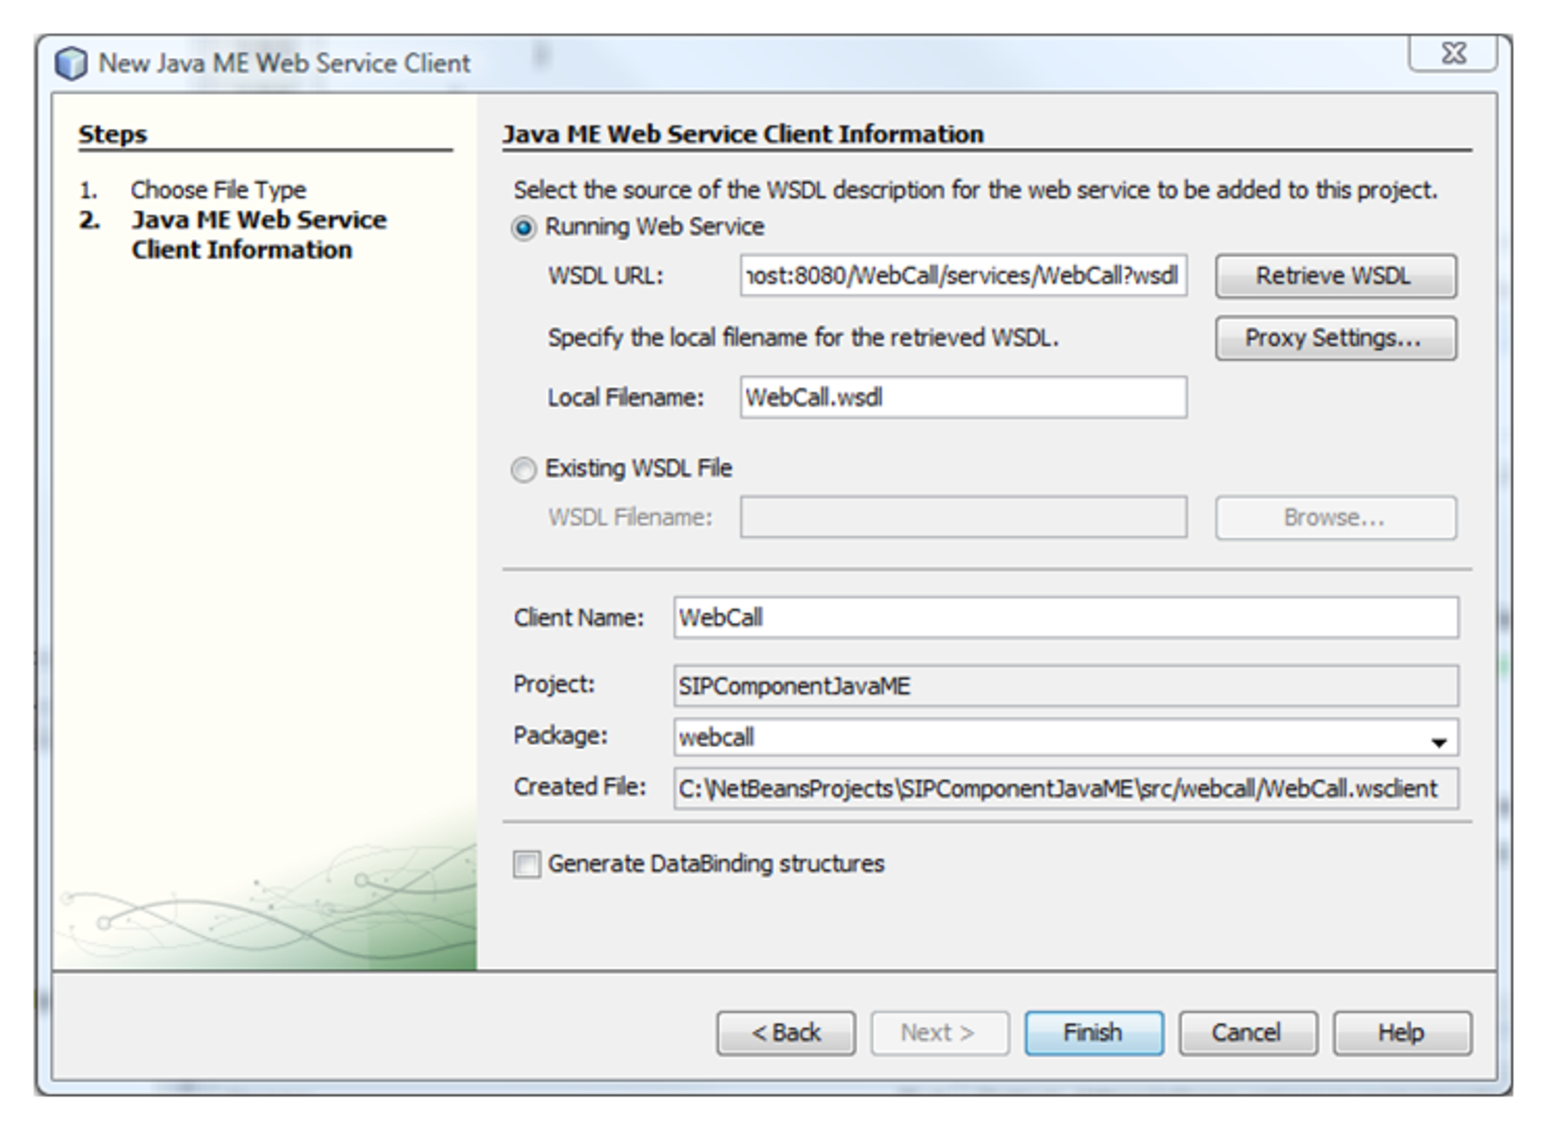
\epsfig{file=chap09/resources/Netbeans_Java_ME_Web_Service_Client_Wizard, width=5.2in}
\caption{Netbeans Java ME Web Service Client Wizard}
\label{fig:NetbeansJavaMEWebServiceClientWizard}
\end{figure}

Once the wizard is finished, NetBeans will automatically generate some classes that wrap the stub and make the operation of web service easily. And it communicates with web service server via SOAP protocol. The web service client stub is designed to be separately from the core logic of Java ME client (Web Service Client). This makes the lower stack of web service exchangeable. As just mentioned above, the client must be installed in a \texttt{JSR 172} enabler. The project team is planning to define a RESTful web service and a RESTful web service client to replace current SOAP based web service client stub. Since The RESTful web service only need a HTTP connection which is widely supported by modern mobile phones, the Java ME client will be installed on more devices by then. 


\section{Record Store Manager}
\label{sec:JavaMEClient:RecordStoreManager}

Record Store Manager is used for reading and writing the data from/to Java ME \textit{record management system} (RMS). It extends a abstract class which named \texttt{AbstractRecordStoreManager} which is a stand alone component which supplies a very convenient way to interactive with RMS. The \texttt{AbstractRecordStoreManager} can be not only used in Java ME Client of Web Call Example Application, but also other Java ME applications. A class hierarchy diagram of \texttt{RecordStoreManager} and \texttt{AbstractRecordStoreManager} is shown in Figure \ref{fig:TheClassDiagramofRecordStoreManager}.

\begin{figure}[!hbtp]
\centering
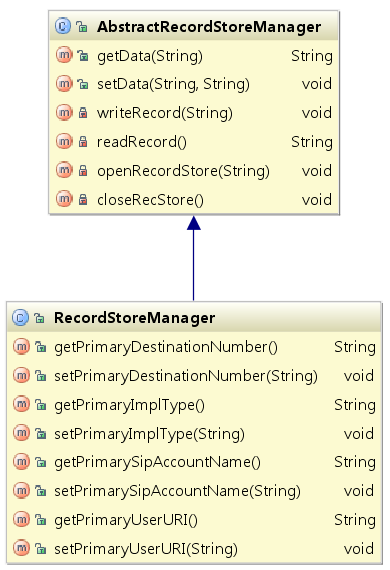
\epsfig{file=chap09/resources/record_store_manager, width=4in}
\caption{The Class Diagram of Record Store Manager}
\label{fig:TheClassDiagramofRecordStoreManager}
\end{figure}

\section{PIM Contact Helper}
\label{sec:JavaMEClient:PIMContactHelper}


\begin{figure}[!hbtp]
\centering
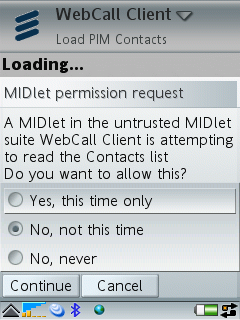
\epsfig{file=chap09/resources/load_pim_contacts, width=3in}
\caption{Load PIM Contacts}
\label{fig:Load PIM Contacts}
\end{figure}


\begin{figure}[!hbtp]
\centering
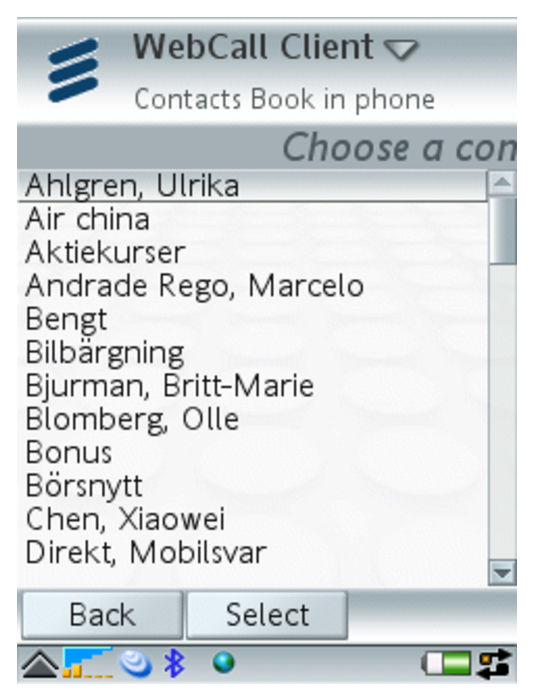
\epsfig{file=chap09/resources/pim_contacts, width=3in}
\caption{PIM Contacts List}
\label{fig:PIMContactsList}
\end{figure}

\section{Web Call Client}
\label{sec:JavaMEClient:WebCallClient}






\section{User Interface}
\label{sec:JavaMEClient:UserInterface}

\begin{figure}[!hbtp]
\centering
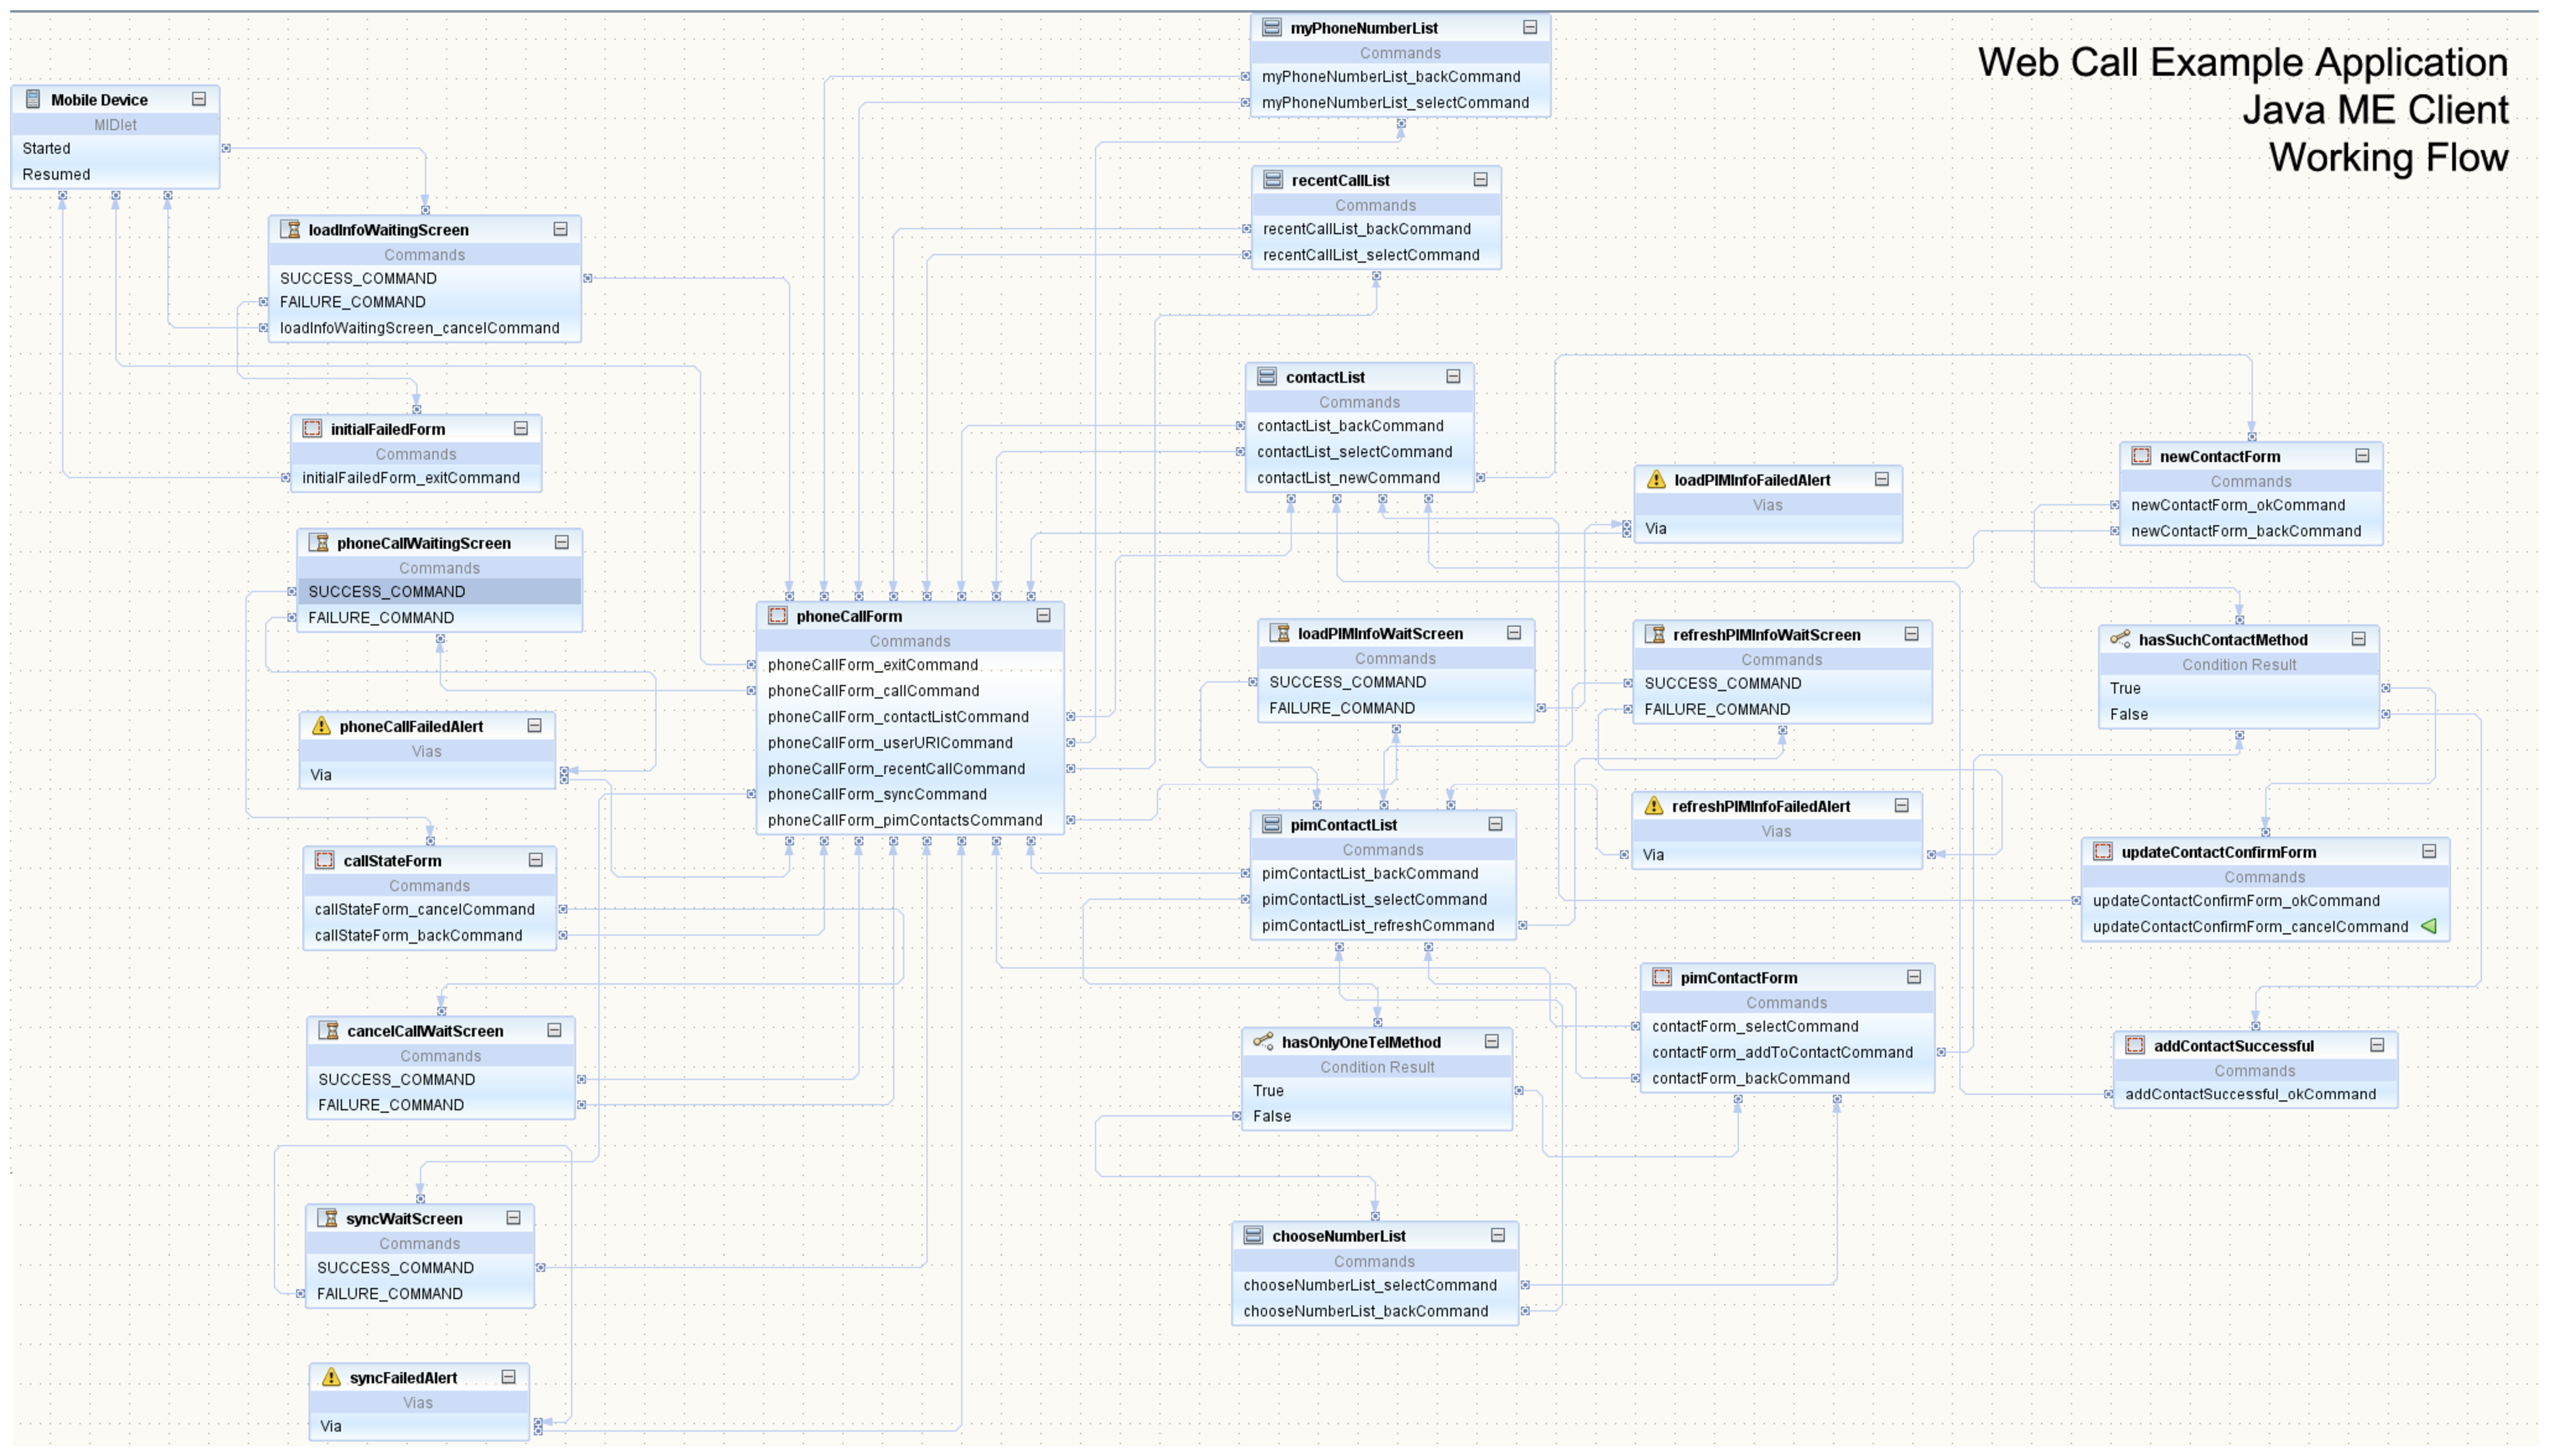
\epsfig{file=chap09/resources/java_me_working_flow, width=8.3in, angle=-90}
\caption{Java ME Client Working Flow}
\label{fig:JavaMEClientWorkingFlow}
\end{figure}

\subsection{VMD-based UI}
\label{sec:JavaMEClient:UserInterface:VMDBasedUI}



\subsection{Java ME Generic UI}
\label{sec:JavaMEClient:UserInterface:JavaMEGenericUI}

\section{Installation of Java ME Client}
\label{sec:JavaMEClient:InstallationOfJavaMEClient}

\section{Security of Java ME Client}
\label{sec:JavaMEClient:SecurityOfJavaMEClient}

% ********** End of chapter **********
